% ================================
% Section 1: Representability
% ================================
\subsection{Accuracy and Representability of the QSE Subspace}
In this section, we study the spectral accuracy and representability of low-lying roots generated with QSE using statevector simulations. 
The QSE excitation energies are compared against exact CASCI energies within the same active space. 
Unless otherwise stated, we focus on the singlet ground state, S0, together with the lowest singlet and triplet excited states, S1, T1 and T2, to characterise QSE performance in the low-energy region of the spectrum.

\subsubsection{Overview of statevector QSE performance}

\begin{figure}[!ht]
    \centering
    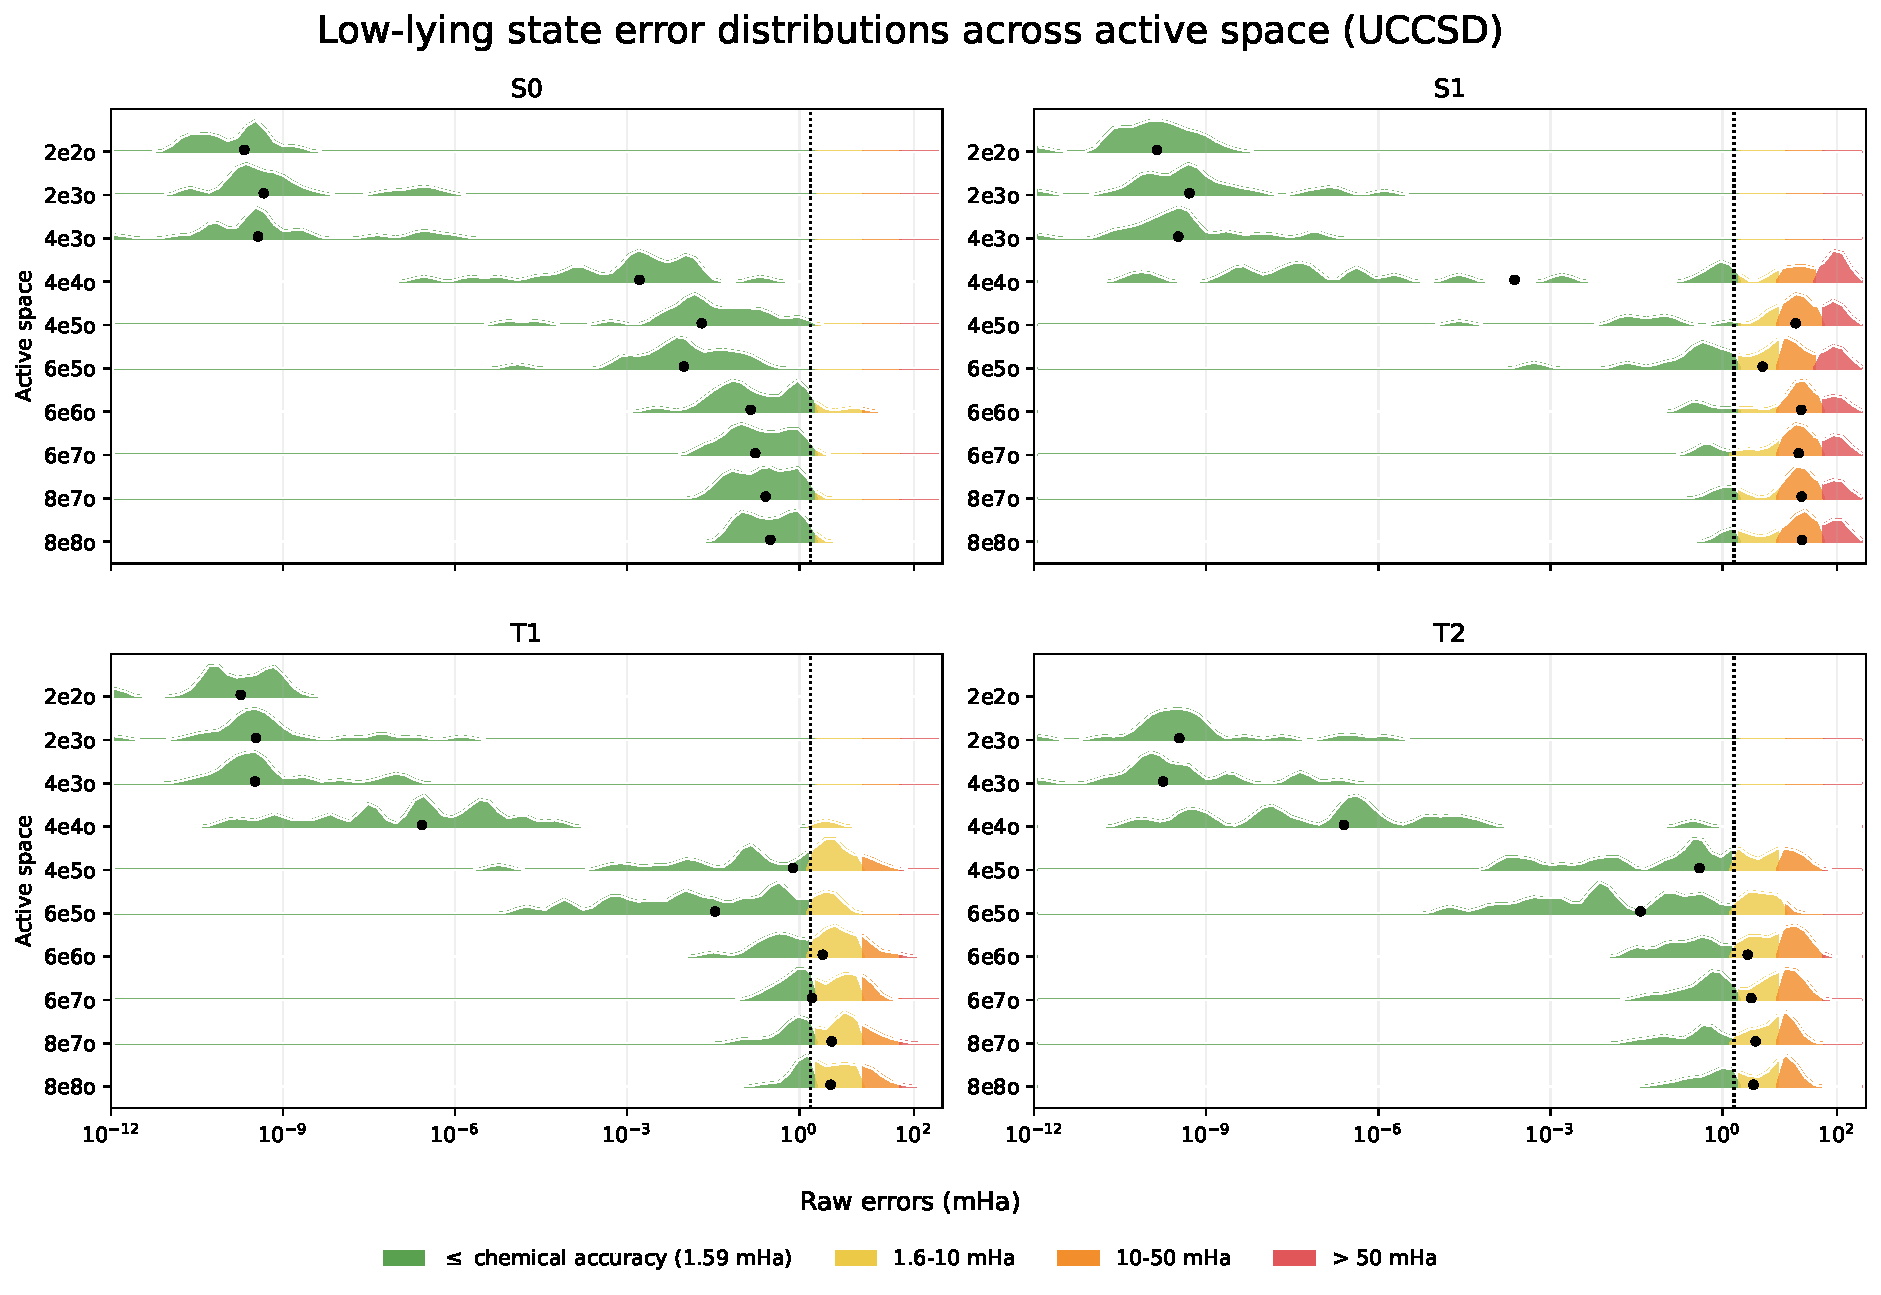
\includegraphics[
        width=\linewidth
    ]{figures/active_space_representability/uccsd_tiered_error_ridgelines.pdf}
    \caption{Distribution of QSE energy errors across the molecular benchmark for the low-lying singlet and triplet states.}
\end{figure}

Across the low-lying states, QSE performance tends to deteriorate as the active space is enlarged. 
For the smallest active spaces, $2e2o$, $2e3o$, and $4e3o$, the recovered spectra are nearly exact. 
Beyond these cases, substantially larger errors are observed across the benchmark. 

The near-exact recovery in the smallest active spaces is consistent with the relative dimensionality of the QSE subspace. 
In these cases, the one-body operator pool generates more basis states than there are physically accessible determinants within the relevant spin sector.
The QSE subspace can therefore span most of the relevant Hilbert space, leaving little room for representability error.
This favourable dimensionality does not persist as the active space grows. The number of one-body QSE operators scales polynomially, approximately as $n^2$, whereas the dimension of the full configuration-interaction (FCI) space grows combinatorially with the number of electrons and orbitals. 
Therefore, the fraction of the many-electron space accessible to the generated QSE subspace decreases with system size, providing a natural explanation for the overall deterioration in accuracy.

However, active-space size alone does not fully account for the observed error trends. 
The deterioration in performance is nonuniform, with a particularly pronounced increase in errors between four and five orbital active spaces. 
Furthermore, active spaces with the same number of orbitals can exhibit markedly different performance even when the relative dimensionality of the QSE and exact spaces is unchanged, as seen most clearly for 4e5o and 6e5o.

Beyond active-space dependent trends, the QSE errors also vary substantially between electronic states. The ground state $S_0$ is generally recovered within chemical accuracy, whereas the lowest lying singlet state $S_1$ exhibits the largest errors. 
The low-lying triplet states $T_1$ and $T_2$ are recovered more accurately than $S_1$, although not consistently within chemical accuracy. 

To further quantify the representability of these states, we define a projection metric
\QSEProjectionEquation
which measures the fraction of the $k$-th exact CASCI state contained within the span of the operator-generated QSE basis states. 
Importantly, this projection is evaluated directly from the operator-generated QSE basis states, before solving the generalised eigenvalue problem. 
It therefore isolates the representability of the target state from subsequent effects associated with overlap-matrix thresholding, numerical conditioning, or the ordering of the recovered Ritz roots.
As shown in \cref{fig:si-error-vs-projection-deficit}, large energy errors are strongly associated with missing projection $1-P_k$. 
This confirms that the observed errors predominantly arise from incomplete representation of the target states within the operator-generated QSE subspace.

\subsubsection{State Dependence of QSE Representability}
Next, we seek to better characterise the state-dependent errors observed above by examining the electronic structure of the exact CASCI states. 
Each CASCI wavefunction is decomposed according to the excitation rank of its constituent Slater determinants relative to the Hartree–Fock (HF) reference. 
We focus in particular on the double-excitation weight, defined as the fraction of the total CI weight arising from determinants that differ from the HF reference by two orbital excitations. 
Doubles are of particular interest because they are the lowest excitation rank not independently represented by the present one-body QSE operator pool. 

The decomposition reveals clear differences between the low-lying states (\cref{fig:si-casci-double-excitation-weight}). 
The $S_1$ states generally exhibit substantial double-excitation weight, whereas the corresponding $T_1$ and $T_2$ states contain markedly smaller contributions. 
This difference is consistent with the closed-shell character of the molecular benchmark. 
Within the double-excitation sector, singlet states can contain both paired and non-pair doubles. 
Triplet states, by contrast, can only obtain double-excitation character from the latter class, since a paired double excitation of a closed-shell HF reference produces another closed-shell singlet determinant. 
The available double-excitaiton manifold is thererfore more restricted for triplet states, consistent with the smaller double-excitation weights observed.

Howeve, it is important to note that double-excitation weight alone does not determine QSE accuracy: $S_0$ contains an even larger doubles contribution while remaining more accurately recovered than the low-lying triplet states. 
This is consistent with the fact that the correlated structure of $S_0$ is already largely encoded in the optimized UCCSD VQE reference, which itself contains double-excitation amplitudes. 

Excited states, however, can require a balance of single and double excitation character that can differ substantially from that of the VQE reference. 
While the one-body operator pool provides independent access to singly excited directions, it does not introduce independent double-excitation directions. 
The corresponding double-excitation amplitudes therefore cannot be tuned independently and remain largely constrained by the VQE reference. 
This reduced flexibility makes excited states with greater double-excitation character generally more difficult to represent accurately within the QSE subspace.

\subsubsection{Molecular Case Studies and Active-Space Effects}
Beyond the broad state-dependent trends, substantial variation in QSE performance is also observed between molecules and across different active spaces for the same molecule. 
We therefore examine several molecular cases to identify the electronic-structure features associated with these deviations.
Since $S_1$ exhibits the largest representability failures across the benchmark, the following case studies focus primarily on this state. 

For each molecule, we first compare the lowest excited QSE root, $q_1$, with the exact CASCI singlet states using wavefunction overlap. 
This diagnostic reveals a particularly consistent pattern for five molecules - butadiene, cyclopentadiene, furan, norbornadiene, and pyrrole. 
For all active spaces $4e4o$ and larger, those five molecules $q_1$ overlaps most strongly with $S_2$ rather than $S_1$ \cref{fig:si-q1-best-root-transition-map}. 
These five molecules all contain 2 C=C double bonds, and their dominant singlet excitation is characterised by a $\pi \rightarrow \pi^{*}$ transition.

Examination of the corresponding CASCI wavefunctions shows that $S_1$ carries substantially stronger double-excitation character, whereas $S_2$ is more strongly dominated by single excitations. 
The restricted one-body QSE subspace therefore represents $S_2$ more readily than the lower-energy $S_1$ state. 
As a result, the poorly represented $S_1$ state is effectively omitted from the recovered spectrum, while the more accessible $S_2$ state appears as the lowest excited QSE root. 
This root omisission accounts for the particularly poor $S_1$ performance of these five molecules, with a mean error of approximately 90mHa. 

\begin{figure}[!ht]
    \centering
    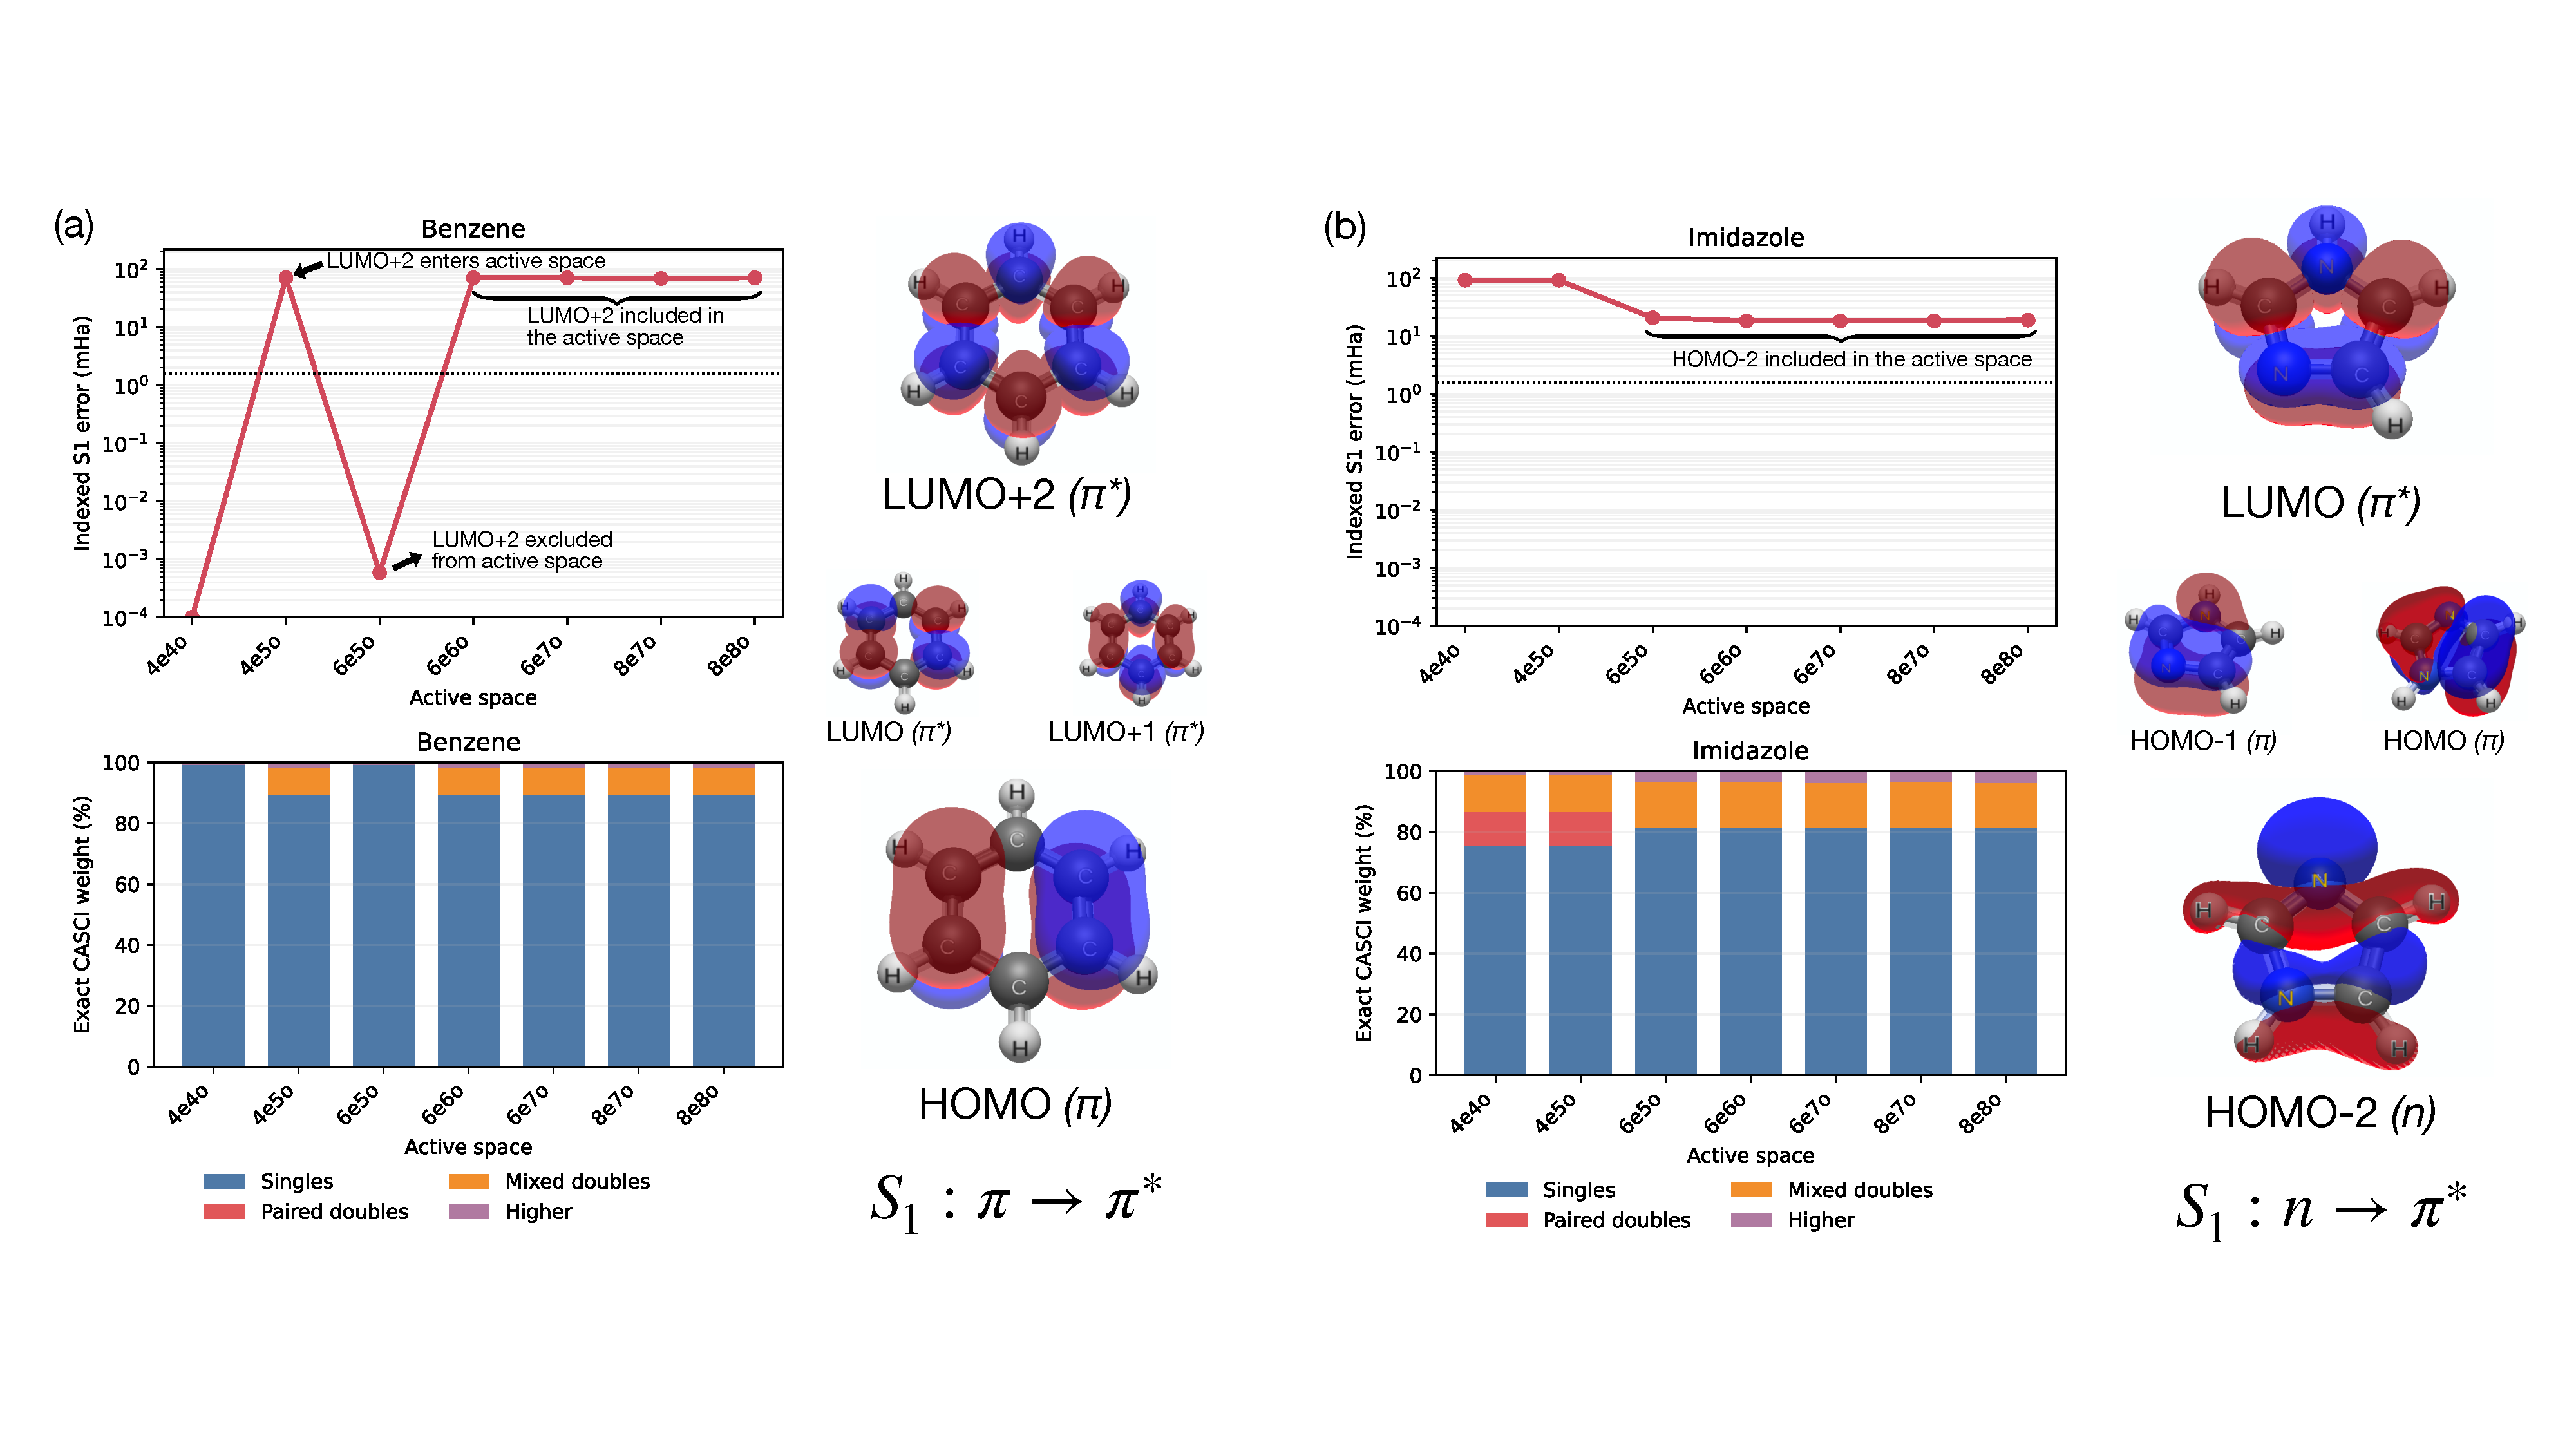
\includegraphics[width=\linewidth]{figures/keynote_figures/case_study_imidazole_benzene.pdf}
    \caption{(a) Benzene case study showing the $S_1$ energy error across active spaces (top left), the corresponding exact $S_1$ wavefunction composition (bottom left), and the relevant frontier molecular orbitals. (b) Corresponding analysis for imidazole.}
    \label{fig:benzene-imidazole-case-studies}
\end{figure}

The molecule-specific variation is also reflected in the sensitivity of QSE performance to the particular orbitals included in the active space. 
Rather than changing smoothly with active-space size, the error can change abruptly when orbitals important to the character of the target state enter the active space.
Benzene provides a prominent example \cref{fig:benzene-imidazole-case-studies}. 
Its low-lying singlet excitation has predominantly $\pi \rightarrow \pi^{*}$ character.
In the more restricted $4e4o$ and $6e5o$ spaces, the exact CASCI states comprise of mainly singly excited determinants, and the $S_1$ errors remain relatively small. 
Once the $LUMO+2$ orbital enters the active space, however, there is an increase in the double-excitation weight of the exact $S_1$ state. 
This results in the QSE errors increasing substantialy.

Imidazole provides a complementary example of the same active-orbital dependence. 
Here, the dominant $S_1$ excitation has $n \rightarrow \pi^{*}$ character, involving the $HOMO-2$ nonbonding orbital and the $LUMO$ \cref{fig:benzene-imidazole-case-studies}.
When $HOMO-2$ is unavailable from the smaller active spaces, this dominant single-excitation is unavailable and the exact state exhibits stronger multiconfigurational character. 
Once $HOMO-2$ enters the active space, the $n \rightarrow \pi^{*}$ excitation becomes directly accessible, and the double-excitation contribution decreases.
This results in a substantial reduction in the QSE error, although not to within chemical accuracy.

Together, these examples show that active-space-dependent variation in QSE accuracy can be traced to the inclusion of specific orbitals that alter the multiconfigurational character of the target state. 
This provides a direct explanation for the pronounced changes in representability observed within the same molecule across different active spaces.

% Ansatz dependence
\subsubsection{Reference Ansatz Dependence of QSE Performance}
We next examine how the choice of variational reference ansatz affects QSE performance. 
Since the QSE subspace is generated from the optimized VQE state, differences in reference quality and excitation flexibility can influence the states accessible to the expansion. 
We therefore compare several UCC-based ansätze with varying levels of expressiveness and circuit complexity.

\label{sec:ansatz-dependence}
\begin{table}[htbp]
    \centering
    \small
    \caption{UCC ansatz complexity and median absolute QSE energy errors for the $6e6o$ active space across the molecular benchmark. Errors are reported in mHa for the lowest singlet ($s0$, $s1$) and triplet ($t1$, $t2$) states.}
    \label{tab:ansatz-errors-6e6o}
    \begin{tabular}{@{}l S[table-format=3.0] S[table-format=5.0] *{4}{S[table-format=2.2]}@{}}
        \toprule
        \multicolumn{3}{c}{Ansatz complexity} & \multicolumn{4}{c}{Median absolute energy error (mHa)} \\
        \cmidrule(lr){1-3} \cmidrule(l){4-7}
        Ansatz & \multicolumn{1}{c}{Parameters} & \multicolumn{1}{c}{Circuit depth} & \multicolumn{1}{c}{$s0$} & \multicolumn{1}{c}{$s1$} & \multicolumn{1}{c}{$t1$} & \multicolumn{1}{c}{$t2$} \\
        \midrule
        1-UpCCGSDSinglet & 30  & 1306  & 17.39 & 35.93 & 6.70 & 23.32 \\
        2-UpCCGSDSinglet & 60  & 2470  & 6.71  & 31.39 & 2.15 & 5.96 \\
        3-UpCCGSDSinglet & 90  & 3634  & 4.14  & 28.23 & 2.65 & 4.30 \\
        UCCSDSinglet    & 54  & 14692 & 0.20  & 23.69 & 2.55 & 3.34 \\
        UCCSD           & 117 & 12249 & 0.14  & 23.69 & 2.79 & 3.17 \\
        UCCGSD          & 315 & 37622 & 0.08  & 22.25 & 1.83 & 2.41 \\
        \bottomrule
    \end{tabular}
\end{table}


We find that QSE performance varies with the choice of reference ansatz, with more expressive ansätze generally producing more accurate QSE spectra. 
The paired k-UpCCGSDSinglet ansatz restricts excitations heavily to only singles and paired doubles. 
Consequently, this ansatz exhibits the largest errors in the predicted spectrum. 
While increasing the number of layers from k=1 to k=3 systematically improves their performance, the ground-state error at k=3 remains more than an order of magnitude larger than that of the next best ansatz. 
This indicates that increasing the flexibility of the paired ansatz does not fully compensate for the restrictions of its excitation manifold.
In comparison, UCCSDSinglet and UCCSD achieve similar accuracies across the low-lying states. 
Although UCCSDSinglet imposes additional parameter-tying constraints, both ansätze span the same excitation manifold, and yield comparable errors.
UCCGSD, which provides the most flexible excitation manifold considered here, generally produces the lowest errors, albeit at the cost of considerably greater circuit depth. 
These results illustrate the expected trade-off between reference-state expressiveness and circuit complexity.

Furthermore, the influence of the reference ansatz is considerably more pronounced for the ground state than for the excited states. 
For S0, the difference in median error between the paired and unpaired ansätze exceeds an order of magnitude, whereas the corresponding variation for S1, T1 and T2 is substantially smaller. 
This difference can be understood from the composition of the exact CASCI states relative to the VQE reference. 
At the $6e6o$ active space, the exact $S_0$ state has a mean squared overlap of $95\%$ with the optimized VQE reference across the six ansätze considered
The ground-state solution therefore depends much more on the quality of the reference wavefunction, and deficiencies in the reference can only be partially corrected by the remaining QSE directions.
In contrast, the maximum squared overlap between the VQE reference and any of the excited states considered remains below $2\%$.
These states therefore rely predominantly on the additional operator-generated directions, whose greater flexibility can partially compensate for imperfections in the reference and reduce their sensitivity to the choice of ansatz.

Beyond spectral accuracy, the choice of reference ansatz also affects the spin purity of the recovered states.
Spin contamination is observed among the recovered QSE roots, with several higher-energy states exhibiting substantial deviations from the target $S(S+1)$ value, in some cases exceeding 1. 
These larger deviations are concentrated predominantly at higher energies, whereas the lowest-lying states remain comparatively less affected (\cref{fig:si-severe-spin-roots}).
Across the ansätze, the more flexible UCCGSD ansatz exhibits the largest degree of spin contamination, whereas the paired ansätze remain nearly spin pure (\cref{fig:si-spin-contaminated-roots}). 
Importantly, we note that imposing spin adaptation at the ansatz level does not necessarily guarantee improved spin purity in the implemented circuit. 
In particular, UCCSDSinglet exhibits greater spin contamination than UCCSD at low Trotter order, an effect associated with finite-order Trotter errors (\cref{tab:s2-spin-mean-trotter})
A more detailed analysis of the spin contamination is provided in \cref{sec:si-spin-purity}.

Taken together with the spectral-error analysis above, these results identify UCCSD as a favourable compromise among the ansätze considered. 
It maintains relatively low spectral errors, exhibits substantially less spin contamination than UCCGSD, and avoids the greater circuit depth associated with the more expressive generalized ansatz.


% ================================
% Section 2: Dimension Analysis
% ================================
\subsection{Stable Dimensions of QSE}
\subsubsection{Eigenvalue Distribution}
\begin{figure}[!ht]
    \centering
    \begin{subfigure}{\linewidth}
        \centering
        \begin{overpic}[width=\linewidth]{figures/dimension_analysis/overlap_eigenvalue_spread/uccsd_6e6o.pdf}
            \put(2,38){\makebox(0,0)[l]{\scriptsize\bfseries (a)}}
        \end{overpic}
        \phantomsubcaption
        \label{fig:eigenvalue-spectrum}
    \end{subfigure}

    \vspace{0.5em}

    \begin{subfigure}{\linewidth}
        \centering
        \begin{overpic}[width=\linewidth]{figures/dimension_analysis/overlap_eigenvector_composition/uccsd_6e6o.pdf}
            \put(2,35){\makebox(0,0)[l]{\scriptsize\bfseries (b)}}
        \end{overpic}
        \phantomsubcaption
        \label{fig:eigenvector-composition}
    \end{subfigure}
    \caption{Structure of the UCCSD overlap matrix in the $6e6o$ active space. The upper panel shows the overlap-eigenvalue spectrum for the singlet and triplet sectors across the molecular benchmark. The lower panel decomposes the corresponding overlap eigenvectors into contributions from occupied-number operators, occupied-to-virtual operators, and other operators.}
    \label{fig:eigenvalue-distribution}
\end{figure}

Having examined the representability and spectral accuracy of the QSE subspace, we next turn to its numerical stability. 
As discussed in the Introduction, very small eigenvalues of the overlap matrix $\mathbf{S}$ can strongly amplify noise, making the generalised eigenvalue problem highly sensitive to perturbations.
Here, we examine the full eigenvalue spectrum of $\mathbf{S}$ (\cref{fig:eigenvalue-spectrum}) to understand why these near-null directions arise in the first place. 

One clear trend that emerges is between the eigenvalue magnitude and the composition of its corresponding eigenvector. 
We first classify the QSE excitation operators into three groups: occupied number operators, occupied-to-virtual (OV) excitations, and the remaining excitation classes. 
Each eigenvector of $\mathbf{S}$ can then be decomposed into basis states corresponding to each category (\cref{fig:eigenvector-composition}). 
One clear trend emerges between the eigenvalue magnitude and the composition of its corresponding eigenvector.
The largest eigenvalues are generally associated with OV-dominated eigenmodes. Singlets additionally contain a strongly supported occupied-number mode, while the remaining operator classes contribute predominantly to smaller-eigenvalue directions. 
For the singlet subspace, this produces one number-dominated eigenvector followed by a block of OV-dominated eigenvectors with eigenvalues close to unity, after which the spectrum drops to progressively smaller values. The triplet subspace retains the OV-dominated stable block, but the corresponding occupied-number contribution is much more weakly supported.

This behaviour can be understood from how the different QSE operators act on the underlying VQE reference. 
Because the reference state is dominated by the Hartree Fock determinant, operators that act directly on this component generate strongly supported basis directions and therefore larger overlap eigenvalues. 
In contrast, operators that annihilate the dominant Hartree Fock component, or act primarily on the smaller correlated components of the reference state, generate much weaker directions and correspondingly smaller eigenvalues.

This operator-support picture also explains the contrasting behaviour of the occupied number operators in the singlet and triplet sectors. As defined in \cref{eq:qse-singlet-operator-pool,eq:qse-triplet-operator-pool}, the diagonal singlet operator for an occupied spatial orbital $i$ is proportional to $\hat n_{i\alpha}+\hat n_{i\beta}$, so that
\SingletOnHFEquation

The dominant Hartree-Fock component therefore provides strong support for this direction, consistent with the large singlet overlap eigenvalues observed. In contrast, the $M_S=0$ triplet diagonal operator is proportional to $\hat n_{i\alpha}-\hat n_{i\beta}$, which gives
\TripletOnHFEquation

The $M_S=\pm1$ diagonal triplet operators likewise annihilate the closed-shell Hartree-Fock determinant because the corresponding spin-flip attempts to create an electron in an already occupied spin orbital. 
The triplet number operators therefore receive support only from configurations containing singly occupied spatial orbitals. 
This is particularly consequential for 1-UpCCGSD, which only allows for singles and paired doubles excitations. Its spectrum, shown in \cref{fig:si-1up-triplet-eigenvalues}, highlights the corresponding $M$ number-operator directions appearing as near-null eigenvalues.

A second source of near-null directions observed occurs within the $2e2o$, $2e3o$, and $4e3o$ active spaces. In those cases, the number of nominal QSE basis states exceeds the dimension of the physically accessible subspace within the relevant spin sector. 
This results in redundant linear combinations, which manifest as near null eigenvalues of the overlap matrix $\mathbf{S}$. 
More generally, this occurs for small active spaces in which the orbital window does not extend beyond $HOMO\pm1$ and $LUMO\pm1$. 
The resulting near-null eigenvalues are therefore not caused by weak operator support alone, but can arise simply from the dimensionality constraint of the many-electron Hilbert space.

\subsubsection{Significance of Small Eigenvalues}
Taken together, these trends reveal a recurring block of comparatively large overlap eigenvalues associated with the strongly supported operator classes identified above.
The corresponding stable dimensions are therefore approximately $1+n_{\mathrm{occ}}n_{\mathrm{vir}}$ for singlets and $3n_{\mathrm{occ}}n_{\mathrm{vir}}$ for triplets, with the remaining directions progressively less well supported. 
We term these dimensions \textit{stable} because their associated overlap eigenvalues remain consistently of order 1 or larger. Retaining these directions therefore does not introduce any strong noise amplifications.

This naturally raises the question of whether these \textit{stable} dimensions alone are sufficient to recover most of the low-energy QSE spectrum. 
This is of significant interest because a consistently stable rank would provide a natural basis for thresholding, particularly when shot-sampling noise is introduced.
To test this, we restrict the QSE subspace to the stable, strongly supported dimensions identified above and solve the resulting generalised eigenvalue problem.
However, restricting the QSE subspace to only these stable dimensions severely degrades the recovered spectrum, producing markedly larger energy errors across the target states (\cref{fig:si-max-stable-error-distribution}).

This suggests that while the stable dimensions form a well-conditioned core of the QSE subspace, they themselves are insufficient to recover the low-lying states accurately.
The remaining weakly supported directions contribute important correlation effects that cannot be trivially discarded.
This establishes a central trade-off: removing weak directions improves numerical stability, but can simultaneously degrade the representability and accuracy of the QSE subspace. 

% ================================
% Section 3: Shots
% ================================
\subsection{Finite-Shot Effects on Generalized Eigenvalue Stability}
This trade-off becomes particularly important under finite-shot sampling, where the near-null region of the overlap spectrum is most strongly perturbed, resulting in the smallest eigenvalues even becoming negative (\cref{fig:si-eigenvalue-lifting}). 
This motivates the use of overlap-eigenvalue thresholding to remove poorly resolved directions.
In this section, we therefore examine how thresholding can be used appropriately to regularise QSE under finite-shot noise.
Sampling-induced errors are reported as the mean absolute deviation of the four low-lying states $S_0$, $S_1$, $T_1$, and $T_2$, from their corresponding statevector QSE energies. 
Unless otherwise stated, $n_{\mathrm{shots}}$ denotes the number of shots allocated to each commuting measurement group.

\subsubsection{Effects of Thresholding to mitigate Sampling Noise}
\begin{figure}[!ht]
    \centering
    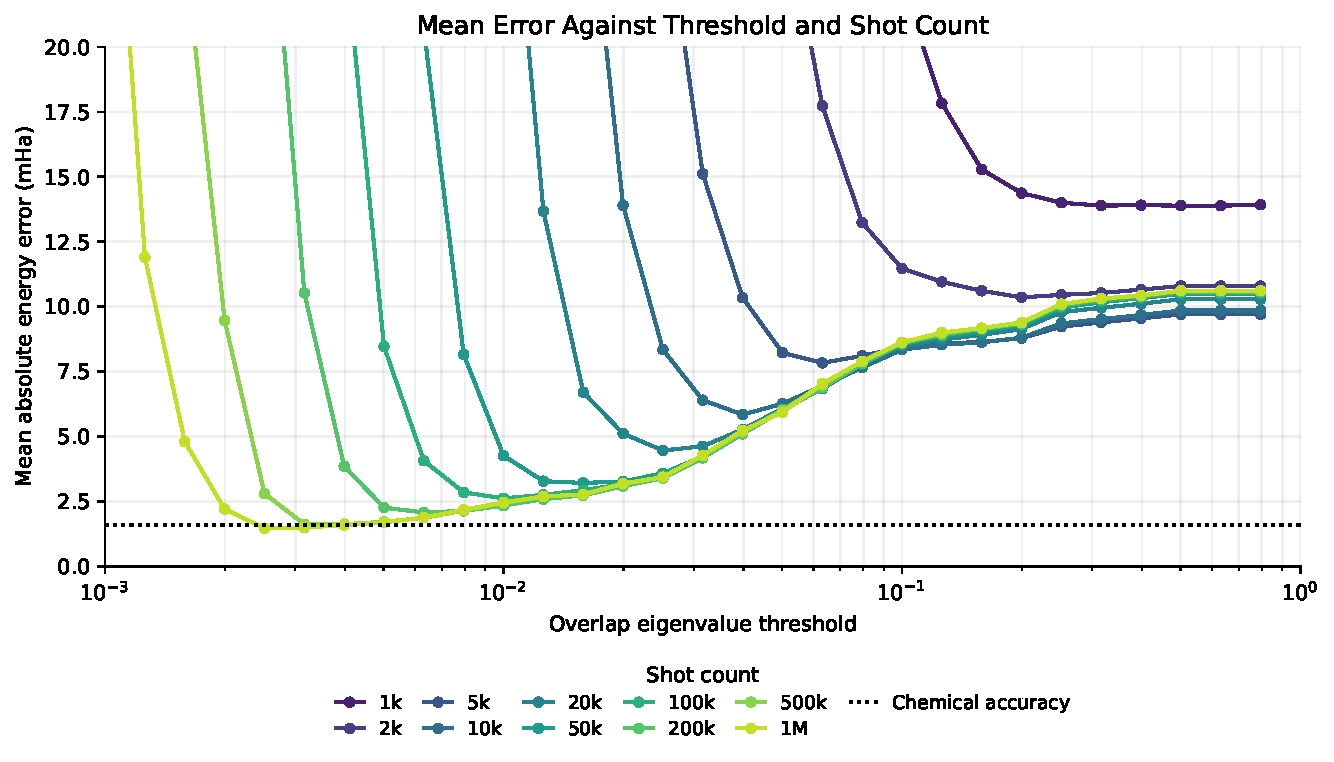
\includegraphics[width=\linewidth]{figures/shots/threshold_shot_error_6e6o.pdf}
    \caption{Mean absolute QSE energy error as a function of the overlap-eigenvalue threshold for the $6e6o$ active space at different shot counts. The dotted line indicates chemical accuracy, and the curves show the trade-off between suppressing sampling-noise amplification and discarding physically relevant subspace directions.}
    \label{fig:threshold-shot-error}
\end{figure}
\Cref{fig:threshold-shot-error} shows a clear minimum in the QSE error as a function of the overlap-eigenvalue threshold, indicating that an optimal degree of regularisation exists for each noise level. 
As the number of shots increases and the sampling noise decreases, this minimum shifts towards lower thresholds and lower overall errors.

This behaviour reflects the competing effects of thresholding. 
Directions associated with very small overlap eigenvalues are particularly susceptible to noise amplification, such that their contribution to the recovered spectrum can become dominated by statistical error rather than useful physical information. 
Increasing the threshold initially removes these poorly resolved directions and therefore reduces the QSE error. 
However, beyond the optimum, further increasing the threshold begins to remove directions that still contain physically important contributions to the QSE subspace, causing the error to increase again. 
The resulting minimum therefore represents a balance between suppressing noise-amplified directions and retaining sufficient information for accurate spectral recovery \cref{fig:si-optimal-threshold}.

Increasing the shot count improves the precision of the projected matrix elements and therefore allows progressively smaller overlap eigenvalues to be resolved reliably. Consequently, fewer directions need to be removed, shifting the optimal threshold towards smaller values as the shot count increases.

\subsubsection{Active Space Dependence of Shot Noise}
\begin{figure}[!ht]
    \centering
    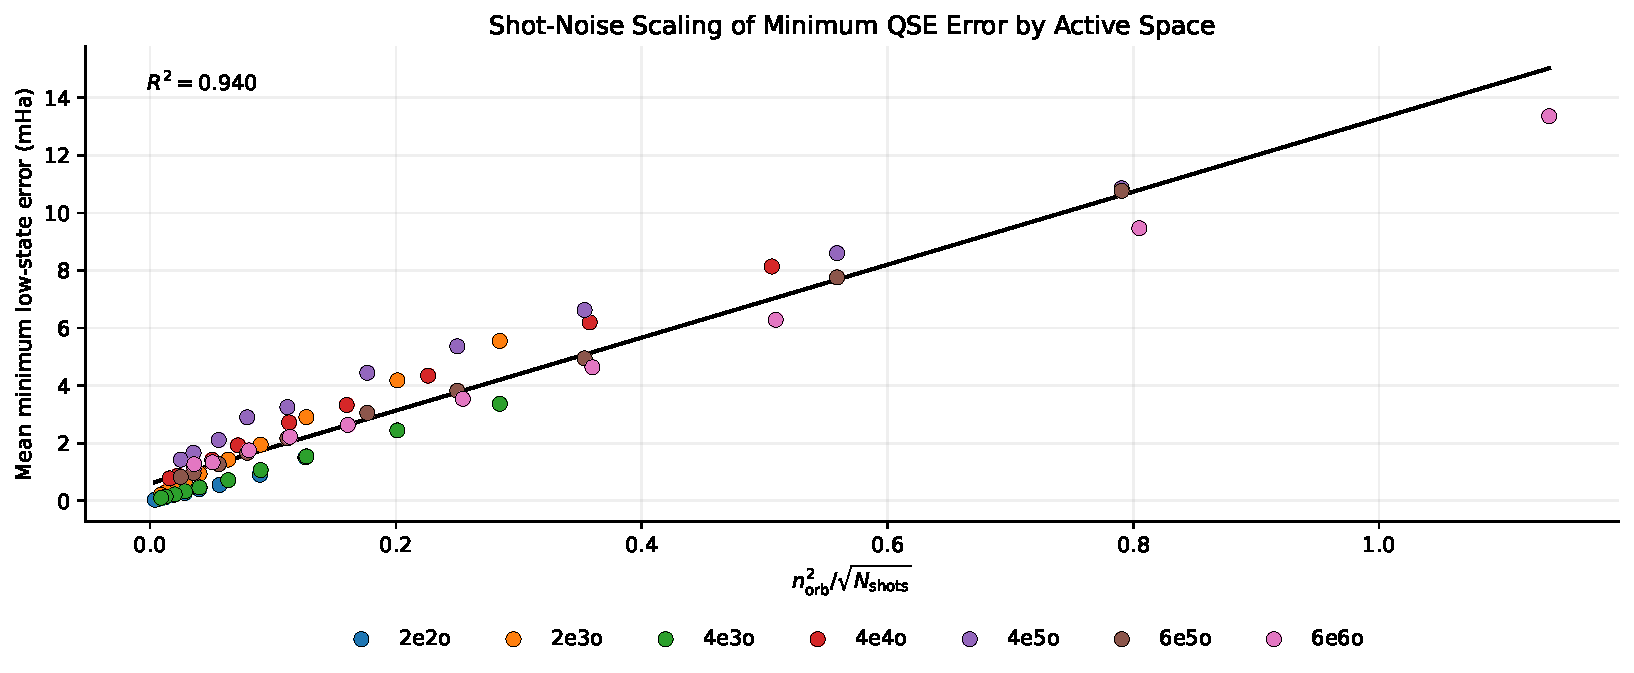
\includegraphics[width=\linewidth]{figures/shots/active_space_shot_scaling_regression.pdf}
    \caption{Threshold-optimised mean low-state QSE energy error as a function of the active-space scaling variable $N_{\mathrm{orb}}^2/\sqrt{N_{\mathrm{shots}}}$. Colours identify the active space, while the black line and annotation show the global linear regression and coefficient of determination.}
    \label{fig:shot-error-scaling}
\end{figure}

We further find that finite-shot errors depend systematically on the size of the QSE projected matrices. 
Empirically, the minimum error after threshold optimisation scales approximately as 
\ErrorScalingEquation
where $n_{\mathrm{orb}}$ is the number of active spatial orbitals (\cref{fig:shot-error-scaling}). 
Consistent with this trend, the optimal overlap threshold generally increases with the active-space size and decreases with shot count (\cref{fig:si-optimal-threshold}).
This indicates that progressively stronger regularisation is required as the projected problem grows or as the sampling precision is reduced. 

This behaviour can be rationalised from the accumulation of finite-sampling errors across the projected matrices. 
The precision of expectation values estimated from $N_{\mathrm{shots}}$ repeated measurements follows a known $N_{\mathrm{shots}}^{-1/2}$ scaling \cite{Knill2007PrecisionScaling}. 
This scaling characterises the errors of each individual matrix element. 
However, as the active spaces grow, the number of matrix elements also increases. For a $d \times d$ projected matrix, the Frobenius norm of the accumulated finite-shot perturbation scales approximately as $\frac{d}{\sqrt{N_{\mathrm{shots}}}}$. 
Perturbation bounds for generalised Hermitian eigenvalue problems relate the generalised-eigenvalue errors to the spectral norms of the perturbations in $\mathbf{H}$ and $\mathbf{S}$ \cite{Nakatsukasa2010ErrorBounds}. 
Since the spectral norm is bounded above by the Frobenius norm, the growth of the accumulated matrix perturbation sets a natural upper scale for the resulting QSE energy errors. 
For the singles-only operator pool used here, the projected-matrix dimension scales as $d \propto n_{\mathrm{orb}}^2$. 
Tthe empirical dependence in \cref{eq:error-scaling} is therefore consistent with the accumulation of finite-shot perturbations as the projected problems grow.
This correspondence should not be interpreted as a direct derivation of the energy-error scaling, but rather as a consistency between the observed empirical trend and the expected growth of matrix perturbations. 
Nevertheless, the averaged low-energy errors are well described by this empirical relationship over the active spaces studied.

\subsubsection{Shot Budget Scaling}
The empirical scaling in \cref{eq:error-scaling} can be used to estimate the measurement requirements for maintaining a fixed QSE accuracy as the active space grows. To maintain a constant error relative to the statevector, this would require approximately $N_{\mathrm{shots}} \propto n_{\mathrm{orb}}^4$. 
For the $6e6o$ active space, recovering states to within chemical accuracy relative to the statevector already requires an excess of $2 \times 10^{5}$ shots per commuting group (\cref{fig:threshold-shot-error}). 

The total measurement cost also depends on the number of distinct commuting groups required to construct both projected matrices. 
Across the active spaces studied, we empirically determine this scaling to be about $\mathcal{O}\!\left(n_{\mathrm{orb}}^{6.77}\right)$ for singlets and $\mathcal{O}\!\left(n_{\mathrm{orb}}^{6.75}\right)$ for triplets (\cref{fig:si-commuting-group-scaling}). 
Here, the number of commuting groups was taken by grouping commuting terms across both matrices, after discarding Pauli terms with coefficients below $10^{-12}$. 

Combining these two contributions gives an estimated total shot requirement for maintaining an approximately constant finite-shot accuracy as
\TotalShotScalingEquation

This empirically derived estimate indicates that QSE has a steep shot measurement overhead. Importantly, the present analysis considers only a one-body operator pool, whose size scales with $\mathcal{O}\!\left(n_{\mathrm{orb}}^{2}\right)$. 
However, the representability results above suggest that more expressive operator pools may be required for chemically accurate excited-state recovery.
Doing so can dramatically increase the shot overhead beyond the estimations we present in \cref{eq:total-shot-scaling}.
For example, including two-body excitation operators would increase the operator-pool size to $\mathcal{O}\!\left(n_{\mathrm{orb}}^{4}\right)$. 
If the observed dependence of finite-shot error on projected-matrix dimension persists, maintaining constant accuracy would then require approximately $\mathcal{O}\!\left(n_{\mathrm{orb}}^{8}\right)$ shots per commuting group. 
The number of required measurement groups would also increase with the enlarged projected problem, leading to an even steeper scaling of the total measurement cost.

% ================================
% Section 4: Future Work
% ================================
\subsection{Scaling and Future Work}
\subsubsection{Addition of Doubles Operators}
% Doubles error
\begin{figure}[htbp]
    \centering
    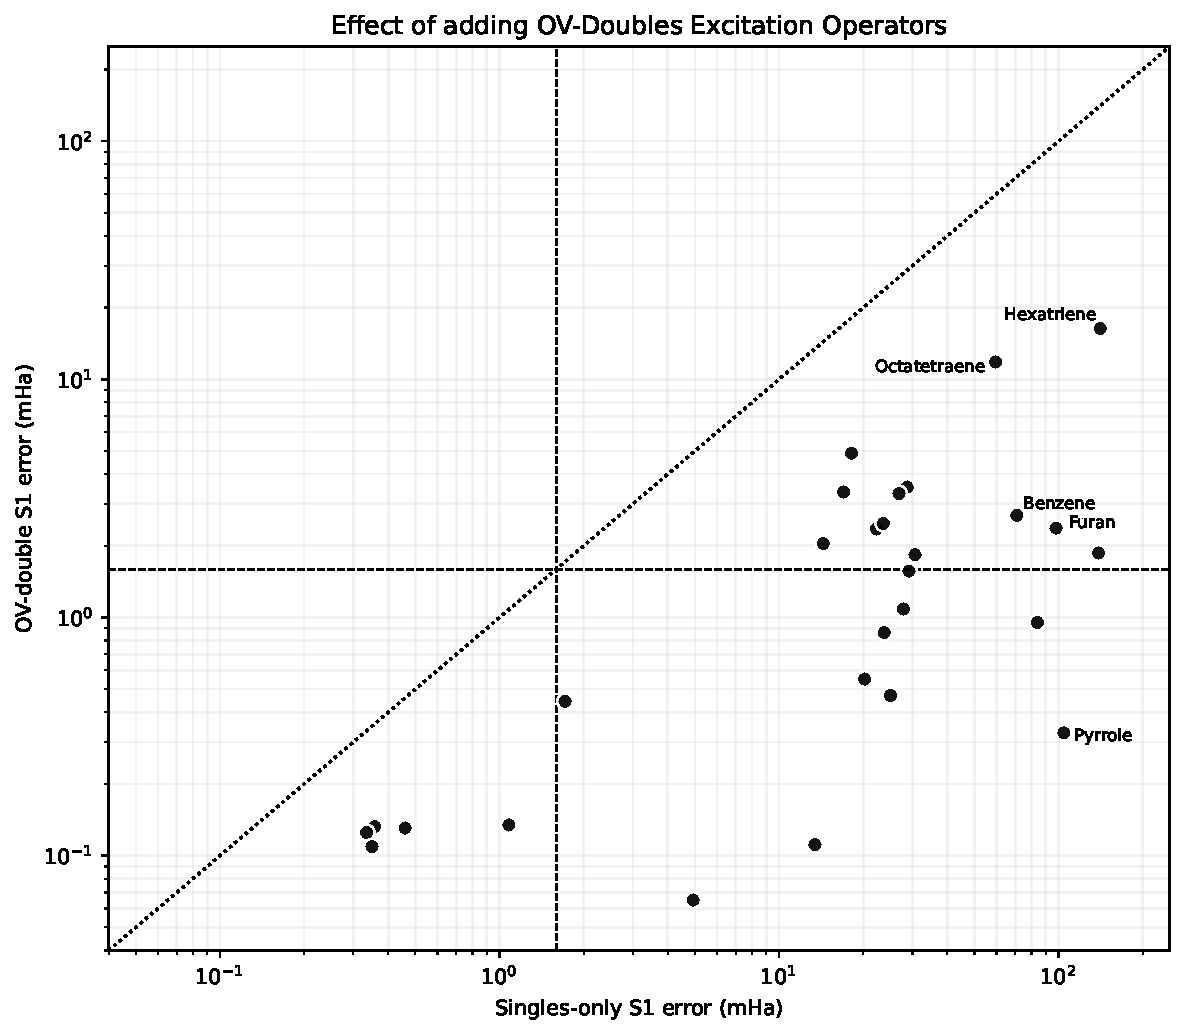
\includegraphics[width=\linewidth]{figures/scaling_future_work/ov_doubles_s1_error_comparison.pdf}
    \caption{Comparison of $S_1$ QSE energy errors obtained with occupied-to-virtual singles and with an expanded operator pool including double excitations.}
    \label{fig:si-ov-doubles-s1-error-comparison}
\end{figure}

% Talk about the effect of adding doubles operators 

While the preceding analysis indicates steep measurement overhead, we find that the projected matrices themselves exhibit substantial structure that may provide opportunities for more efficient reconstruction. 
In this section, we examine the recurring patterns and correlations within the projected $\mathbf{H}$ and $\mathbf{S}$ matrices, and how these features are affected by finite-shot sampling.

\subsubsection{Structural Correlations and Sparsity}
We first observe a strong correlation between corresponding elements of the projected $H$ and $S$ matrices (\cref{fig:si-h-s-element-correlation}). In general, elements with small overlap $S_{ij}$ also tend to have small Hamiltonian couplings $H_{ij}$ and vice versa. 
This suggests that the Hamiltonian predominantly couples pairs of operator-generated states that already have appreciable overlap within the QSE subspace.

The matrices also exhibit pronounced internal structure. The overlap-matrix heatmaps in \cref{fig:si-full-singlet-heatmaps,fig:si-full-triplet-heatmaps} show consistently large diagonal elements, as expected from the self-overlap of the operator-generated states. 
The off-diagonal elements are much less uniform. 
Stronger couplings instead appear in recurring block-like regions associated with particular classes of excitation operators, leaving other regions weakly coupled or nearly empty.
Consequently, the degree of sparsity varies substantially between matrices.
Interestingly, however, we find no clear relationship between this sparsity and the molecular properties considered across the benchmark. 
This suggests that the observed coupling patterns are not determined by molecular identity alone, but also depend on the chosen active space and the orbitals included within it. 
Regardless of the degree of sparsity, the QSE matrix elements exhibit clear structure rather than being uniformly distributed.

\subsubsection{Effects of Noise on Structure}
\begin{figure}[!ht]
    \centering
    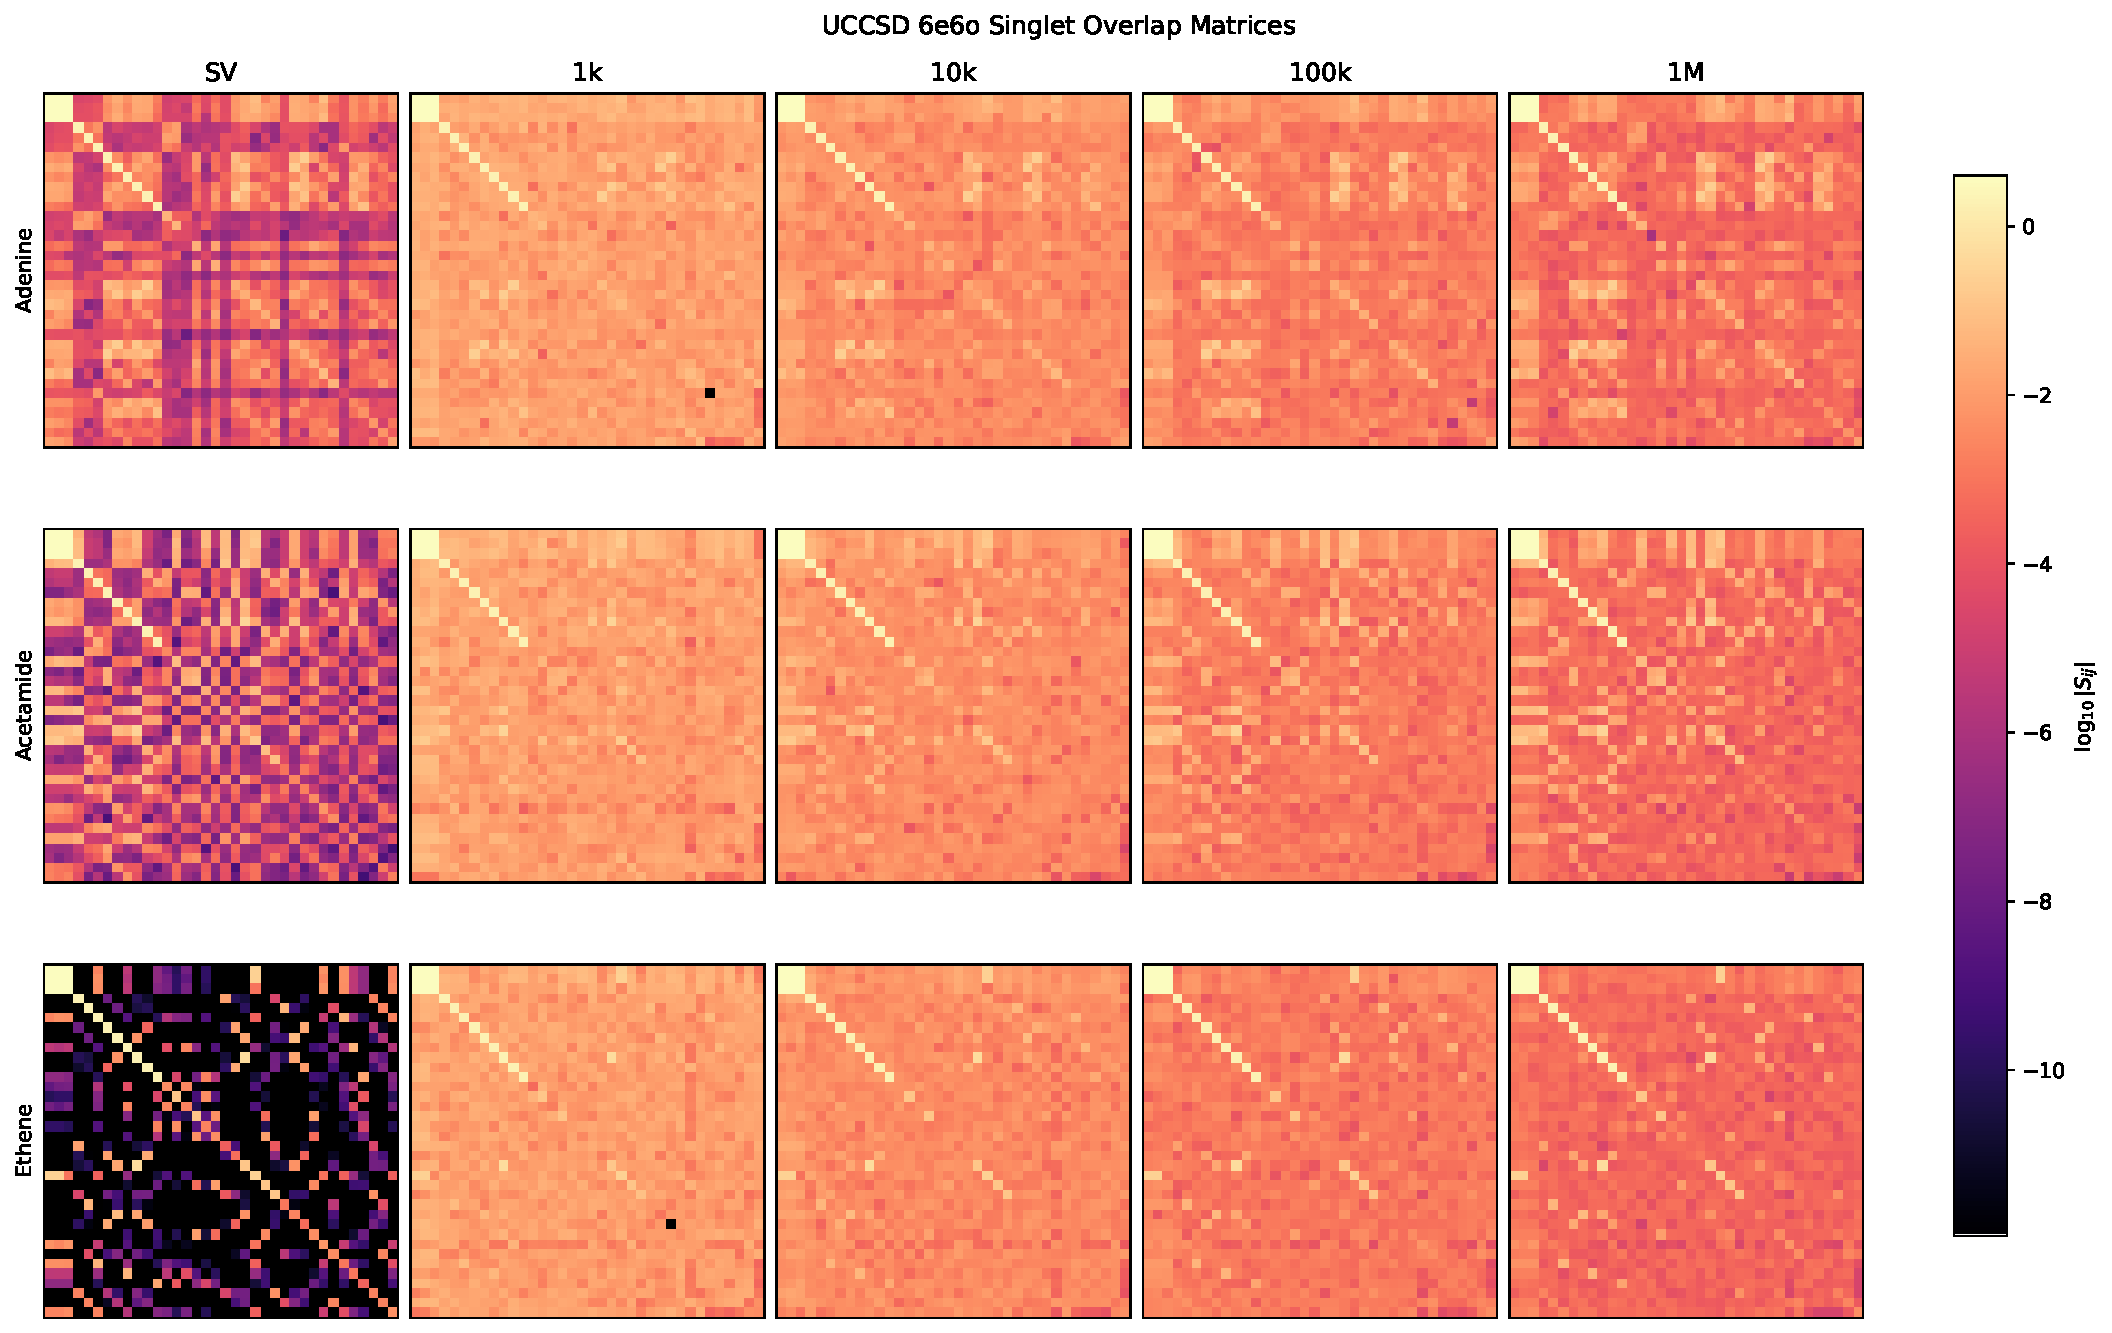
\includegraphics[width=\linewidth]{figures/scaling_future_work/matrix_heatmaps/uccsd_6e6o_shot_overlap.pdf}
    \caption{Effect of finite-shot noise on the structure of UCCSD overlap matrices in the $6e6o$ singlet sector. The statevector matrix is compared with matrices reconstructed using shot counts from $1\,\mathrm{k}$ to $1\,\mathrm{M}$, illustrating the progressive disruption of the underlying matrix structure by sampling noise.}
    \label{fig:shot-overlap-structure}
\end{figure}

We next consider how finite-shot sampling affects the matrix structure identified above. 
As shown in \cref{fig:shot-overlap-structure}, sampling noise progressively obscures the detailed patterns present in the statevector overlap matrices. 
The dominant diagonal elements remain visible even at relatively low shot counts, whereas the finer off-diagonal and block-like structures are substantially blurred. 
Increasing the number of shots gradually restores these features, with the reconstructed matrices approaching the underlying statevector structure more closely at higher sampling precision.

Importantly, these finite-shot perturbations should not be interpreted as independent random errors applied to each matrix element. 
In our measurement procedure, Pauli terms are grouped globally across the projected matrices, such that the same sampled measurement outcomes contribute to multiple matrix elements. 
The resulting errors are therefore expected to exhibit correlations across the reconstructed matrices. 
This provides an additional source of structure in the finite-shot problem beyond that already present in the underlying statevector matrices.

\subsubsection{Outlook for Structure-Aware reconstruction}
The observations above suggest that finite-shot QSE should not simply be treated as a problem of reconstructing two dense matrices from independent noisy estimates. 
The corresponding elements of $\mathbf{H}$ and $\mathbf{S}$ are strongly correlated, the statevector matrices exhibit recurring internal structure, and the finite-shot perturbations themselves are expected to be correlated through the shared measurement groups. 
As such, the projected QSE problem is highly structured at both the signal and noise levels.

We envisage that this structure may provide opportunities for classical post-processing methods to reconstruct the projected matrices more accurately from a limited number of measurements. 
Related approaches have already been explored in quantum error mitigation, where machine-learning and model-based methods exploit systematic structure or correlations in noisy measurement data to improve estimates of ideal observables \cite{Liao2024MLQEM, Aasen2025ReadoutMitigation}. 
These methods are effective because the targeted errors are not treated as completely independent fluctuations, but instead contain patterns that can be learned or explicitly modelled. 

As such, the steep shot scaling identified above should therefore be interpreted as the cost of the present direct-estimation strategy. 
Structure-aware reconstruction methods that exploit the features we identified may allow comparable spectral accuracy to be achieved with substantially fewer measurements.
